%%
%
% ARQUIVO: main.tex
%
% VERSÃO: 1.1
% DATA: Janeiro de 2016
% AUTOR: Coordenação PPgSC
% 
%  Arquivo tex principal do documento de Dissertação.
%  Este arquivo SÓ PRECISA SER MODIFICADO NA PARTE DE CONTEÚDO:
%
%    a. colocar um \include{•} para cada capítulo da Dissertação.
%
%%

% -----
% CLASSE DO DOCUMENTO DA PROPOSTA DE DISSERTAÇÃO
% -----
\documentclass{proposta}

% -----
% PACOTES LATEX USADOS NO DOCUMENTO DA PROPOSTA DE DISSERTAÇÃO
% -----
\usepackage[brazilian]{babel}
\usepackage[utf8]{inputenc}
\usepackage[T1]{fontenc}

\usepackage{amsmath}
\usepackage{graphicx}
\usepackage{tabularx}
\usepackage{float}
\usepackage{color}
\usepackage{amsfonts,amssymb}
\usepackage[authoryear]{natbib}

\usepackage{enumitem}
\usepackage{rotating}
\usepackage{lipsum}
\usepackage{lastpage}
\usepackage{stringstrings}
\usepackage{pgffor}

% -----
% MARGENS DO DOCUMENTO DA PROPOSTA DE DISSERTAÇÃO
% -----
\usepackage{geometry}
\geometry{
	a4paper,
	total={210mm,297mm},
	left=25mm,
	right=25mm,
	top=25mm,
	bottom=30mm,
	textwidth=160mm,
	textheight=242mm,
	headheight=0mm,
	headsep=0mm,
}

% -----
% DECLARAÇÕES AUXILIARES PARA REFERÊNCIAS
%
%  Diferencia \citet e \citep de acordo com a NBR 10520:2002
% -----
\DeclareRobustCommand{\NATand}{;}
\DeclareRobustCommand{\NATetal}{et~al.}
\makeatletter
\renewcommand{\NAT@nmfmt}[1]{%
  \ifNAT@swa\expandafter\MakeUppercase
  \else\DeclareRobustCommand{\NATand}{ e}\expandafter\@firstofone\fi{{\NAT@up #1}}%
}
\makeatother

% -----
% AMBIENTE DE FIGURAS DA PROPOSTA DE DISSERTAÇÃO
%
%  A classe do documento está configurada SOMENTE para figuras no formato EPS.
%  Logo, use PREFERENCIALMENTE este tipo de arquivo.
%
%    a. os arquivos das figuras devem estar no diretório 'img'
% -----
\graphicspath{{./img/}}

% -----
% INÍCIO DO DOCUMENTO DA PROPOSTA DE DISSERTAÇÃO
% -----
\begin{document}

% -----
% DADOS DA PROPOSTA DE DISSERTAÇÃO
%  ALTERAR o arquivo dados-proposta.tex
% -----
%%
%
% ARQUIVO: dados-proposta.tex
%
% VERSÃO: 1.1
% DATA: Janeiro de 2016
% AUTOR: Coordenação PPgSC
% 
%  Arquivo tex com os dados acerca da Proposta de Dissertação.
%
%
%%

%%% AUTOR DA PROPOSTA DE DISSERTAÇÃO (Nome completo)
\autor{Seu Nome Completo}

%%% CÓDIGO DO AUTOR DA PROPOSTA DE DISSERTAÇÃO
\codigoautor{SC XXXXX}

%%% POSTO DO AUTOR DA PROPOSTA DE DISSERTAÇÃO
% ---
%  se o autor é CIVIL, REMOVA ESTA LINHA
%  se o autor é MILITAR, coloque CORRETAMENTE o POSTO aqui
% ---
%\postoautor{1 Ten}

%%% TITULO DA PROPOSTA DISSERTAÇÃO
\titulo{Título Completo da Proposta de Dissertação}

%%% DATA DA APRESENTAÇÃO (formato {dd}{Mmmmm}{aaaa})
\dataapresentacao{31}{Fevereiro}{2016}

%%% ÁREA DE CONCENTRAÇÃO DA PROPOSTA DISSERTAÇÃO
% ---
%  VER SITE do PPGSC para ver as Áreas de Concentração do Programa.
%  Em 2016 só existe uma Área de Concentração:
%     Ciência da Computação
% ---
\area{Área de Concentração da Proposta de Dissertação}

%%% LINHA DE PESQUISA DA PROPOSTA DISSERTAÇÃO
% ---
%  VER SITE do PPGSC para ver as Linhas de Pesquisa do Programa.
%  Em 2016 só existem três Linhas de Pesquisa:
%     Metodologia da Computação
%     Sistemas de Computação
%     Engenharia de Sistemas e Informação
% ---
\linha{Linha de Pesquisa da Proposta de Dissertação}

%%% ORIENTADOR DA PROPOSTA DE DISSERTAÇÃO
% ---
%  CAMPO 1: Nome completo
%  CAMPO 2: D (para D.Sc.); P (para Ph.D.); ou qualquer coisa (inclusive VAZIO) - o que for escrito aparecerá no documento
% ---
\orientador{Nome Completo do Orientador}{D}

%%% POSTO DO ORIENTADOR DA PROPOSTA DE DISSERTAÇÃO
% ---
%  se o orientador é CIVIL, REMOVA ESTA LINHA
%  se o orientador é MILITAR, coloque CORRETAMENTE o POSTO aqui:
%     pode ser: 1 Ten; Cap; Maj; Ten Cel; Cel
% ---
\postoorientador{Ten Cel}

%%% CO-ORIENTADOR DA PROPOSTA DE DISSERTAÇÃO
% ---
%  se NÃO HOUVER co-orientador, REMOVA ESTA LINHA
%  preenchimento idêntico a \orientador{}{}
% ---
%\coorientador{Nome Completo do Co-orientador}{P}

%%% POSTO DO CO-ORIENTADOR DA PROPOSTA DE DISSERTAÇÃO
% ---
%  se NÃO HOUVER co-orientador, REMOVA ESTA LINHA
%  caso contrário
%    se o co-orientador é CIVIL, REMOVA ESTA LINHA
%    se o co-orientador é MILITAR, coloque CORRETAMENTE o POSTO aqui:
%       pode ser: 1 Ten; Cap; Maj; Ten Cel; Cel
% ---
%\postocoorientador{Cap}

%%% COORDENADOR DE PÓS-GRADUAÇÃO
% ---
%  CAMPO 1: Nome completo
%  CAMPO 2: D (para D.Sc.); P (para Ph.D.); ou qualquer coisa (inclusive VAZIO) - o que for escrito aparecerá no documento
% ---
\coord{Nome Completo do Coordenador}{P}

%%% POSTO DO COORDENADOR DE PÓS-GRADUAÇÃO
% ---
%  se o Coordenador de PG é CIVIL, REMOVA ESTA LINHA
%  se o Coordenador de PG é MILITAR, coloque CORRETAMENTE o POSTO aqui:
%     pode ser: 1 Ten; Cap; Maj; Ten Cel; Cel
% ---
\postocoord{Cel}

%%% CHEFE DA SEÇÃO (SE/8)
\chefe{Nome Completo do Chefe da SE/8}

%%% POSTO DO CHEFE DA SEÇÃO (SE/8)
% ---
%  se o Chefe é CIVIL, REMOVA ESTA LINHA
%  se o Chefe é MILITAR, coloque CORRETAMENTE o POSTO aqui:
%     pode ser: 1 Ten; Cap; Maj; Ten Cel; Cel
% ---
\postochefe{Cel}



% -----
% PARTE PRÉ-TEXTUAL DA PROPOSTA DE DISSERTAÇÃO
% -----
\makecapa
\maketitle

\parindent 0.75cm


% -----
% PARTE DE CONTEÚDO DE SUA PROPOSTA DE DISSERTAÇÃO
%
% Alterar o conteúdo dos arquivos capitulo-02.tex / capitulo-03.tex / capitulo-04.tex
% -----
% -----
% ARQUIVO: capitulo-02.tex
% VERSÃO: 1.1
% DATA: Janeiro de 2016
%
% CAPÍTULO DE INTRODUÇÃO DA PROPOSTA
%
% NÃO MEXA NAS SEÇÕES, SOMENTE EDITE O CONTEÚDO.
% -----

\chapter{Introdu\c{c}\~{a}o}
% #TXT_INTRODUCAO
Introdução do trabalho aqui

\section{Motiva\c{c}\~{a}o}
% #TXT_MOTIVACAO
Estudo tem relevância tanto para o mercado, academia e para o governo. Detalhar o papel do exército na defesa cibernética do país. 

Motivação: Delay entre atualização dos sistemas de malware e a analise do especialista
problema da escolha de característica



\subsection{Caracteriza\c{c}\~{a}o do Problema}
% #TXT_PROBLEMA

Curse of dimentionality? \\
Pre treinamento nao supervisionado\\
Autoencoders\\
Deep learning.

% -----
% ARQUIVO: capitulo-03.tex
% VERSÃO: 1.1
% DATA: Janeiro de 2016
%
% CAPÍTULO DE CONCEITOS BÁSICOS DA PROPOSTA
%
% NÃO MEXA NAS SEÇÕES, SOMENTE EDITE O CONTEÚDO.
% -----

\chapter{Conceitos B\'{a}sicos e Estado da Arte}
% #TXT_CONCEITOS
\textbf{Explicando Malware\\
Explicando técnicas de análise de malware: Estática, Dinâmica, Híbrida\\
Explicando técnicas de evasão(?)\\
Explicando Deep Learning\\\\
Entrar no estado da arte para deep learning e análise de malware separadamente ou no caso aqui o estado da arte é Análise de malware com deep learning?}


% Para usar figuras, use sempre o mesmo template abaixo. altere somente:
% 1. os parâmetros do comando \includegraphics[width=•]{•} / tamanho e arquivo
% 2. \caption{*} / para colocar o rótulo da figura em *
% 3. \label{*} / para colocar a chamada para a figura no texto em *
%    TODA figura deve ter uma chamada no texto e esta deve ser feita sempre no formato:
%    Figura \ref{•} (p. ex. "Figura \ref{fig:artigo1}")

\begin{figure}[!h]
	\centering
	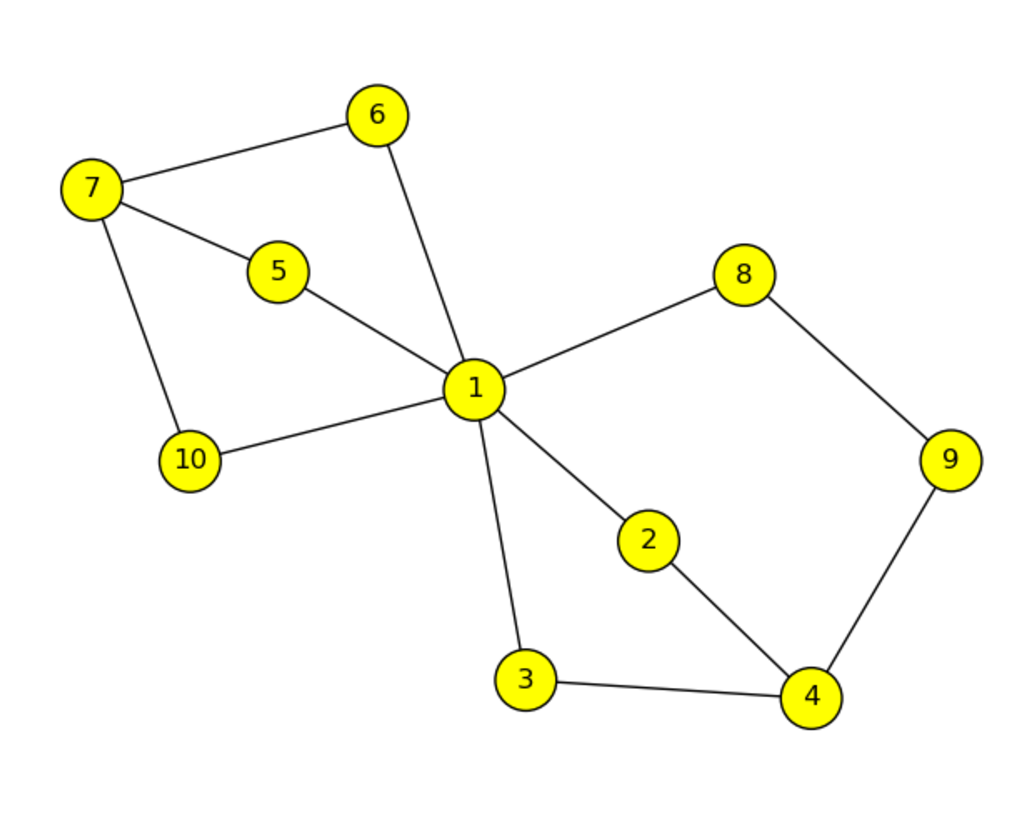
\includegraphics[width=0.4\textwidth]{artigo1.eps}
	\caption{R\'{o}tulo da Figura 1, descrevendo a figura.}
	\label{fig:artigo1}
\end{figure}

\section{Trabalhos Relacionados}
% #TXT_TRABREL
\textbf{Definir paragrafo inicial:} Explicar os problemas da análise de malware: Descrever sobre o gargalo gerado por necessitarmos de um analista especialista para realizar a análise de um arquivo, criando uma demora na atualização dos sistemas de segurança.  Informar que a velocidade que os malwares são criados e alterados, utilizando-se de diversas técnicas de evasão, criam a necessidade de ferramentas automatizadas mais inteligentes e adaptáveis não só aos malwares conhecidos mas também a novos malwares. Mostrar a necessidade da pesquisa na área é cada vez mais importante, visto que agora o potêncial dos danos é ainda maior, já que temos cada vez mais dispositivos com boa capacidade de processamento e acesso a redes rápidas, como smartphones e outros dispositivos (internet das coisas, por exemplo).
Explicar um pouco como o deep learning poderia ajudar na tarefa de extração de característica e criação da hierarquia de representações a partir de dados brutos sem a necessidade de um especialista. Detalhar os trabalhos relacionados (somente deep learning)

Diversos estudos vem sendo conduzidos tanto em inteligência artificial, no desenvolvimento de algoritmos de treinamento e novas arquiteturas de redes neurais com o objetivo de aprender essas hierarquias de representações, tanto em análise de malware, preocupando-se em criar sistemas mais robustos e resistentes às técnicas de evasão empregadas por códigos maliciosos. Também podemos observar vários trabalhos que se utilizaram de técnicas de Deep Learning aplicadas ao problema da análise de malware, seja por análise estática, dinâmica ou híbrida. Abaixo, comentamos um pouco sobre esses trabalhos. 

\subsection{Trabalhos com foco em Análise de Malware}
Trabalhos com foco em análise de malware aqui

\subsection{Trabalhos com foco em Deep Learning}
Trabalhos com foco em deep learning aqui

\subsection{Trabalhos com Deep Learning aplicado à Análise de Malware}
Trabalhos com foco em Analise de Malware com aplicação de tecnicas de deep learning aqui

INCLUIR TABELA COM MEDIDAS AQUI

%
% Ambiente de teoremas: \begin{*}
% * pode assumir os seguinte valores:
%	1. thm  - Teorema (na sequência, o texto aparece em itálico)
%	2. prop - Proposição
%	3. defn - Definição (na sequência, o texto aparece em itálico)
%	4. exmp - Exemplo
%	5. nota - Nota
%
\begin{thm}
Um Teorema simples:
\begin{equation}
X^2 := x^2 - 123
\label{thm1}
\end{equation}
\end{thm}

\lipsum[13] 

%
% Referência para um teorema (é igual para todas as opções do ambiente de teoremas)
Conforme o Teorema \ref{thm1}, nemo enim ipsam voluptatem quia voluptas sit aspernatur aut odit aut fugit, sed quia consequuntur magni dolores eos qui ratione voluptatem sequi nesciunt. Neque porro quisquam est, qui dolorem ipsum quia dolor sit amet, consectetur, adipisci velit, sed quia non numquam eius modi tempora incidunt ut labore et dolore magnam aliquam quaerat voluptatem. Ut enim ad minima veniam, quis nostrum exercitationem ullam corporis suscipit laboriosam, nisi ut aliquid ex ea commodi consequatur? Quis autem vel eum iure reprehenderit qui in ea voluptate velit esse quam nihil molestiae consequatur, vel illum qui dolorem eum fugiat quo voluptas nulla pariatur?



% -----
% ARQUIVO: capitulo-04.tex
% VERSÃO: 1.1
% DATA: Janeiro de 2016
%
% CAPÍTULO DE METODOLOGIA DA PROPOSTA
%
% NÃO MEXA NAS SEÇÕES, SOMENTE EDITE O CONTEÚDO.
% -----

\chapter{A Proposta}
% #TXT_INTROPROPOSTA
\lipsum[1]

\section{Objetivos e Quest\~{o}es de Pesquisa}
% #TXT_OBJETIVO
\lipsum[1-2]

% PARTE DE QUESTÕES DE PESQUSA - TANTAS QUANTO NECESSÁRIO
\begin{qpesq}
Lorem ipsum dolor sit amet, consectetur adipiscing elit, sed do eiusmod tempor incididunt ut labore et dolore magna aliqua?
\end{qpesq}

\subsection{Hip\'{o}teses}
% #TXT_HIPOTESE
\lipsum[1]

% PARTE DE HIPÓTESES DE PESQUSA - TANTAS QUANTO NECESSÁRIO
\begin{hipo}
Lorem ipsum dolor sit amet, consectetur adipiscing elit, sed do eiusmod tempor incididunt ut labore et dolore magna aliqua?
\end{hipo}

\section{Contribui\c{c}\~{o}es Esperadas}
% #TXT_CONTRIBUICAO
As contribui\c{c}\~{o}es esperadas para este trabalho s\~{a}o:

\begin{enumerate}[label=(\roman*)]
\item Neque porro quisquam est, qui dolorem ipsum quia dolor sit amet, consectetur, adipisci velit, sed quia non numquam eius modi tempora incidunt ut labore et dolore magnam aliquam quaerat voluptatem.

\item At vero eos et accusamus et iusto odio dignissimos ducimus qui blanditiis praesentium voluptatum deleniti atque corrupti quos dolores et quas molestias excepturi sint occaecati cupiditate non provident, similique sunt in culpa qui officia deserunt mollitia animi, id est laborum et dolorum fuga.
\end{enumerate}


% -----
% ARQUIVO: capitulo-05.tex
% VERSÃO: 1.0
% DATA: Agosto de 2015
%
% CAPÍTULO DE PLANO DE AÇÃO DA PROPOSTA
%
% NÃO MEXA NAS SEÇÕES, SOMENTE EDITE O CONTEÚDO.
% -----

\chapter{Plano de A\c{c}\~{a}o}
% #TXT_PLANO
\lipsum[1]

\section{Metodologia}
% #TXT_METODOLOGIA
\lipsum[11]

% Para usar tabelas, use sempre o mesmo template abaixo. Altere somente:
% 1. \caption{*} / para colocar o rótulo da tabela em *
% 2. \begin{tabular}{*} / para colocar a formatação da tabela em *
% 3. o conteúdo da tabela (tudo até \end{tabular})

\begin{table}[h]
\centering
\caption{Um nome qualquer}
\vspace{0.5cm}
\begin{tabular}{r|lr}
 
Posi\c{c}\~ao & Pa\'is & IDH \\ % Note a separação de col. e a quebra de linhas
\hline                               % para uma linha horizontal
1 & Noruega        & .955 \\
2 & Austr{\'a}lia  & .938 \\
3 & EUA            & .937 \\
4 & Holanda        & .921 \\
5 & Alemanha       & .920            % não é preciso quebrar a última linha
 
\label{tab:tabela1}
\end{tabular}
\end{table}

At vero eos et accusamus et iusto odio dignissimos ducimus qui blanditiis praesentium voluptatum deleniti atque corrupti quos dolores et quas molestias excepturi sint occaecati cupiditate non provident, similique sunt in culpa qui officia deserunt mollitia animi, id est laborum et dolorum fuga (como mostrado na Tabela \ref{tab:tabela1}). Et harum quidem rerum facilis est et expedita distinctio. Nam libero tempore, cum soluta nobis est eligendi optio cumque nihil impedit quo minus id quod maxime placeat facere possimus, omnis voluptas assumenda est, omnis dolor repellendus. Temporibus autem quibusdam et aut officiis debitis aut rerum necessitatibus saepe eveniet ut et voluptates repudiandae sint et molestiae non recusandae.

\section{Cronograma}
\lipsum[11]

O cronograma para o desenvolvimento das atividades relacionadas a esta proposta pode ser visto na Figura \ref{fig:cronograma}.

% Para usar figuras, use sempre o mesmo template abaixo. altere somente:
% 1. os parâmetros do comando \includegraphics[width=•]{•} / tamanho e arquivo
% 2. \caption{*} / para colocar o rótulo da figura em *
% 3. \label{*} / para colocar a chamada para a figura no texto em *
%    TODA figura deve ter uma chamada no texto e esta deve ser feita sempre no formato:
%    Figura \ref{•} (p. ex. "Figura \ref{fig:cronograma}")

% #CRONOGRAMA
\begin{figure}[!h]
	\centering
	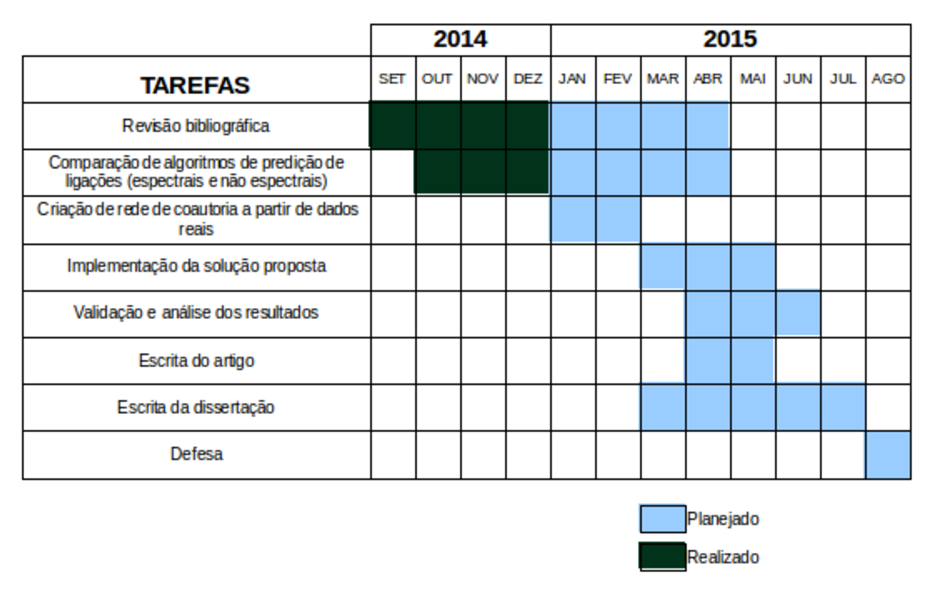
\includegraphics[width=0.9\textwidth]{cronograma.eps}
	\caption{Cronograma da Proposta de Disserta\c{c}\~{a}o.}
	\label{fig:cronograma}
\end{figure}





% -----
% PARTE DE REFERÊCIAS BIBLIOGRÁFICAS DA DISSERTAÇÃO
%
%  As referências da Proposta de Dissertação devem estar no arquivo refs.bib
%  Devem seguir o formato bibtex - ver Manual-Referencias.pdf para mais detalhes.
% -----
\bibliographystyle{proposta}
\bibliography{refs}


% -----
% PARTE DE ASSINATURAS DE SUA PROPOSTA DE DISSERTAÇÃO
% -----
\preparatitulos
\makeassinaturas


% -----
% FIM DO DOCUMENTO DE SUA PROPOSTA DE DISSERTAÇÃO
% -----
\label{theend}
\end{document}
